\pdfoutput=1
\documentclass[10pt,twocolumn,letterpaper]{article}

\PassOptionsToPackage{table}{xcolor}

\IfFileExists{cvpr.sty}{%
  \usepackage{cvpr}%
}{%
  \usepackage[margin=0.75in,top=1in,bottom=1in]{geometry}%
  \setlength{\columnsep}{0.3125in}%
}

\usepackage{times}
\usepackage{graphicx}
\usepackage{amsmath,amssymb}
\usepackage{booktabs}
\usepackage{multirow}
\usepackage{rotating}
\usepackage{xcolor}
\usepackage{array}
\usepackage{colortbl}
\usepackage{microtype}

\definecolor{odfmlink}{rgb}{0.07,0.41,0.66}
\usepackage[pagebackref,breaklinks,colorlinks]{hyperref}
\hypersetup{linkcolor=odfmlink,citecolor=odfmlink,urlcolor=odfmlink}
\usepackage[capitalize]{cleveref}

\graphicspath{{figs/}}

\newcommand{\Hii}{+0.0484}
\newcommand{\HiiCI}{[+0.0390,\,+0.0584]}
\newcommand{\objObs}{0.7623}
\newcommand{\objMSP}{0.7193}
\newcommand{\objDelta}{+0.0432}
\newcommand{\objDeltaCI}{[+0.0135,\,+0.0708]}
\newcommand{\objOracle}{0.7745}
\newcommand{\voxMSP}{0.8797}
\newcommand{\voxObs}{0.6321}
\newcommand{\frmConf}{0.8618}
\newcommand{\frmObs}{0.8066}
\newcommand{\missHi}{47.3\%}
\newcommand{\missLo}{4.7\%}
\newcommand{\nObj}{40{,}863}
\newcommand{\nFrames}{3{,}008}
\newcommand{\nScenes}{75}
\newcommand{\splitdigest}{\texttt{924a44db544d4818}}
\newcommand{\fullpx}{965.0}

\def\paperID{0000}
\def\confName{CVPR}
\def\confYear{2027}

\newcommand{\nMvoFrames}{60}
\newcommand{\nMvoRev}{3}
\newcommand{\nMvoRatio}{$2.6\times$}
\begin{document}

\title{SightOcc: Geometric Observability for Missed Objects\\
       in Camera-Only 3D Occupancy}

\author{%
Akila Lourdes Miriyala Francis \qquad Akilan Manivannan\\
Long Island University, Brooklyn, NY\\
{\tt\small akilalourdes.miriyalafrancis@my.liu.edu}\quad
{\tt\small akilan.manivannan@my.liu.edu}
}

\date{}
\maketitle

\begin{abstract}
\itshape
Camera-only 3D occupancy models are evaluated as though every voxel were
equally observable, yet a model can assign maximal confidence to free
space exactly where the camera rig supplies almost no geometric evidence:
a missed object and correctly observed empty road are both simply
\emph{free}. We introduce {\upshape\textsc{SightOcc}}, a learning-free continuous
measure of \emph{geometric observability} $O(v;\mathcal{G})$ that combines
projected voxel coverage with first-hit visibility across the rig. Unlike
a binary camera-observation mask it carries evidence \emph{strength} and
resolves occlusion explicitly, and on Occ3D-nuScenes it ranks per-voxel
error above the dataset's own \texttt{mask\_camera} flag by \Hii\ AUROC on
a sealed test split. Our main finding is an inversion across granularity.
For whether an individual voxel is wrong, the model's own confidence
dominates geometry (\voxMSP\ against \voxObs). For whether a whole
\emph{object} is missed entirely, geometry wins (\objObs\ against
\objMSP, \objDelta\ over \nObj\ objects) and comes within noise of a LiDAR
point-count oracle. Confidence is a statement about a prediction that was
made, and is structurally unable to flag one that was never made at all.
Because the measure reads external scene geometry, we position it as an
evaluation-time diagnostic.
\end{abstract}

\section{Introduction}

\begin{figure*}[t]
\centering
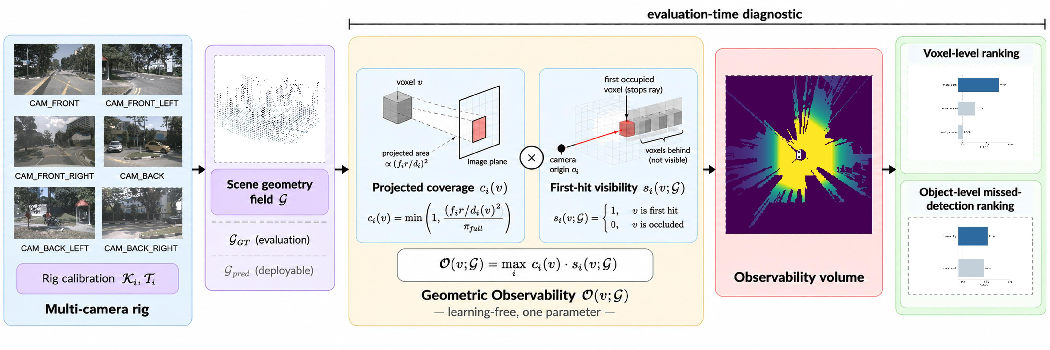
\includegraphics[width=\textwidth]{fig0_hero.pdf}
\caption{\textbf{\textsc{SightOcc}: geometric observability from the camera
rig alone.} The six rig images and the calibration define, for every voxel,
a projected coverage $c_i(v)$ --- how much image area the voxel subtends in
camera $i$ --- and a first-hit visibility $s_i(v;\mathcal{G})$ --- whether
the ray from that camera reaches it through the scene-geometry field
$\mathcal{G}$. Their product, maximised over cameras, is
$O(v;\mathcal{G})$. No training and one parameter. Nothing in the pipeline
reads the occupancy model, which is why the measure can rank failures the
model's own confidence cannot: at object granularity observability reaches
\objObs\ AUROC against \objMSP\ for confidence, while at voxel granularity
the ordering is the other way round. Rig images, geometry volume and
observability map are one sealed-test frame, token
\texttt{312cd4d3}; the two bar panels are the full test split.}
\label{fig:hero}
\end{figure*}

\begin{figure*}[t]
\centering
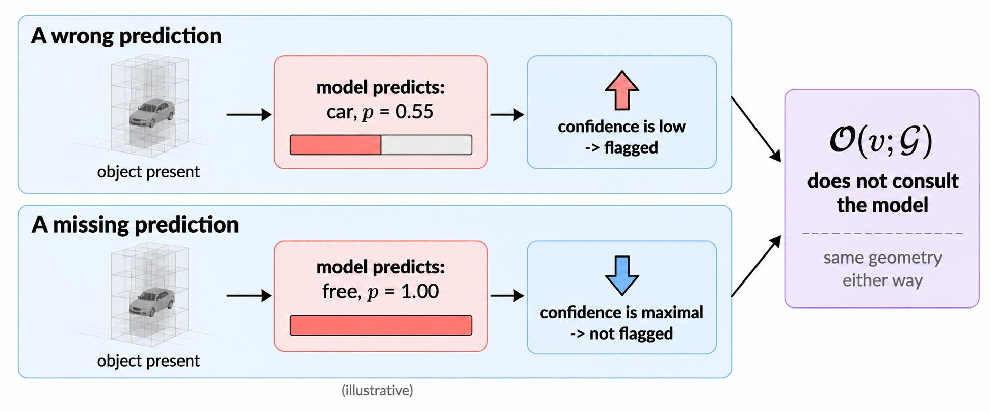
\includegraphics[width=0.92\textwidth]{fig_whyconf.pdf}
\caption{\textbf{Confidence can only rate a prediction that exists.} A
wrong prediction leaves a low-confidence trace, so softmax flags it. A
\emph{missing} prediction leaves a maximally confident vote for
\texttt{free}, which is indistinguishable from correctly observed empty
road, so softmax cannot flag it at all. Geometric observability never
consults the model, so the two cases are identical to it and the second one
is still visible. Probabilities are illustrative; the measured version of
this argument is \cref{tab:perclass} and \cref{fig:quadrant}.}
\label{fig:whyconf}
\end{figure*}

A camera-only occupancy model asked about a volume of space it cannot see
does not abstain. It predicts free space, and it does so confidently.
Nothing in the model's output distinguishes ``there is nothing here'' from
``I have no evidence either way'', because both arrive as a high-probability
vote for the free class. On the held-out scenes used throughout this paper,
\missHi\ of annotated dynamic objects standing in volumes with no camera
evidence are not predicted by the model at all. \Cref{fig:hero} shows one of them.

This matters because of what consumes the occupancy field. End-to-end
planners read occupancy and its descendants as a statement about the
world~\cite{hu2023uniad, chen2024vadv2} and are benchmarked on how well
they act on it~\cite{dauner2024navsim}, and the functional-safety framing
for exactly this hazard class --- a system behaving as designed on input it
was never equipped to interpret --- has its own
standard~\cite{iso21448}. A planner reads the field as a statement about
the world, not as a statement about the camera rig:
a cell marked free is a cell the vehicle may drive through. The
representation has no channel in which to say \emph{I have no evidence
here}, so absence of evidence is delivered to the planner as evidence of
absence, and the planner has no way to tell the two apart. On the frames we
measure, $76.6\%$ of ground-truth obstacle voxels lie in volumes with no
camera evidence at all.

The usual answer is to calibrate the model's own confidence. We show this
answer is adequate for one question and structurally inadequate for
another, and that the boundary between them is the granularity of the
thing being asked about.

Our claim is sharper than ``uncertainty estimation is hard'':
\emph{a score computed from the network's output cannot by itself
distinguish a confidently empty location from a confidently missed object.} A missed
object is not a low-confidence prediction that the right machinery could
surface. It is a confident prediction of the free class, which is
indistinguishable, in the output alone, from correctly observed empty road.
Calibration rescales confidences; it does not create a prediction that was
never made. If the claim is right, the remedy cannot come from the model,
and has to come from something that knows about the sensors.

\paragraph{Two different questions.} Confidence asks whether the
prediction the model just produced is likely to be correct. Observability
asks whether the sensor configuration could have supplied evidence about
that location at all. The two coincide when the model predicts an object
and diverge when it confidently predicts free space, because in that case
there is no object hypothesis whose confidence could be evaluated. No
recalibration of the output changes this: calibration rescales the
confidences attached to predictions that exist. That is the gap external
geometric evidence might fill, and the rest of this paper measures whether
it does.

We therefore propose \emph{geometric observability}, a measure computed
outside the network from the camera rig and a scene-geometry field:
\begin{enumerate}\itemsep0pt
\item it is a function of the camera rig, the ego pose and the scene's
      occupancy, and of nothing the network produces, so it is unchanged
      when the model changes and transfers between architectures;
\item it is continuous, where the dataset's \texttt{mask\_camera} flag is
      binary, so it is constant over the support where we
      compare and cannot rank within it; and
\item it carries exactly one parameter, fixed once at \fullpx\ and never
      retuned per model or per split.
\end{enumerate}

\paragraph{Contributions.}
\begin{itemize}\itemsep0pt
\item \textbf{Geometric observability.} A continuous, learning-free,
      sensor-side measure combining projection coverage with first-hit
      visibility under an \emph{explicit} scene-geometry field
      $\mathcal{G}$, for ranking camera-only occupancy failures.
\item \textbf{The granularity inversion.} Across \nObj\ dynamic objects,
      confidence dominates voxel-level error ranking while observability
      becomes the stronger signal for objects the model never predicts at
      all. The two remain non-redundant at matched confidence.
\item \textbf{The geometry-source boundary.} The object-level advantage
      depends on external scene geometry and collapses when the model's own
      dense occupancy is substituted as the occluder, through
      over-occlusion rather than any circularity in the idea, which
      places the measure at evaluation time and says precisely why.
\end{itemize}


\begin{figure}[t]
\centering
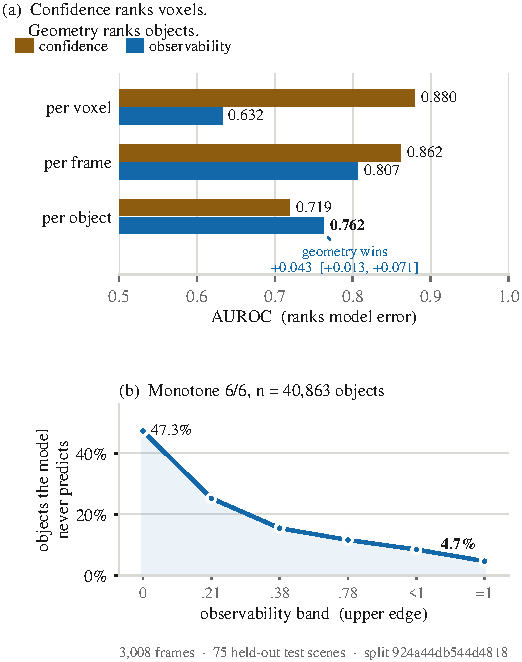
\includegraphics[width=\linewidth]{fig1_granularity.pdf}
\caption{\textbf{Confidence ranks voxels; geometry ranks objects.}
(a)~AUROC for ranking model error at three granularities on the sealed
test split. The model's own confidence dominates geometry per voxel and
per frame, then \emph{loses} per object. (b)~The mechanism: the fraction
of annotated dynamic objects the model never predicts, against
observability, monotone across all six bands over \nObj\ objects.
Confidence cannot flag what the model never predicted.}
\label{fig:teaser}
\end{figure}


\begin{figure*}[t]
\centering
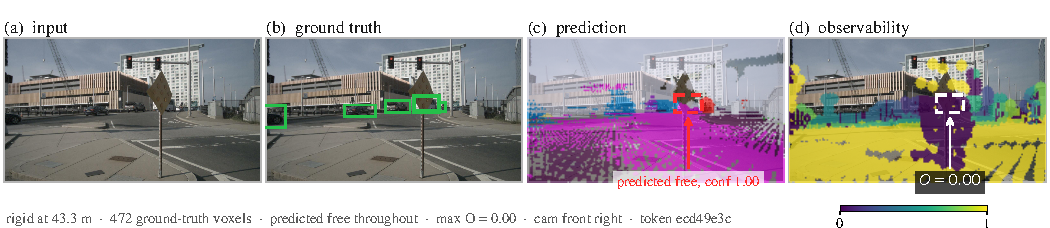
\includegraphics[width=\textwidth]{fig2_qualitative.pdf}
\caption{\textbf{A whole bus, predicted as free space, with maximal
confidence.} One sealed-test frame, token \texttt{ecd49e3c}, in image space.
(a)~The camera the object falls in. (b)~Occ3D ground truth, dynamic boxes
projected; the rigid bus at 43.3\,m, thick box, occupies 472 annotated
voxels. (c)~FB-OCC's predicted occupancy over the same volume, nearest
surface, coloured by class: no dynamic class is predicted anywhere inside
that box and the model assigns \emph{free} there at confidence $1.00$.
Softmax offers no signal, because a confident prediction of free is exactly
what a missed object looks like. (d)~Geometric observability sampled on the
ground-truth surface. The marked region is the darkest in the frame,
$O=0.00$, while the open road either side of it saturates. The geometry
knows the volume is unobserved before the network runs, and knows it
without ever reading the network's output.}
\label{fig:qualitative}
\end{figure*}

\section{Related Work}

Three literatures meet here. One supplies the model whose failures we
study, one supplies the baseline we compare against, and one supplies the
quantity we compute. None of them asks whether sensor geometry ranks
failures better than the network's own confidence.

\begin{figure*}[t]
\centering
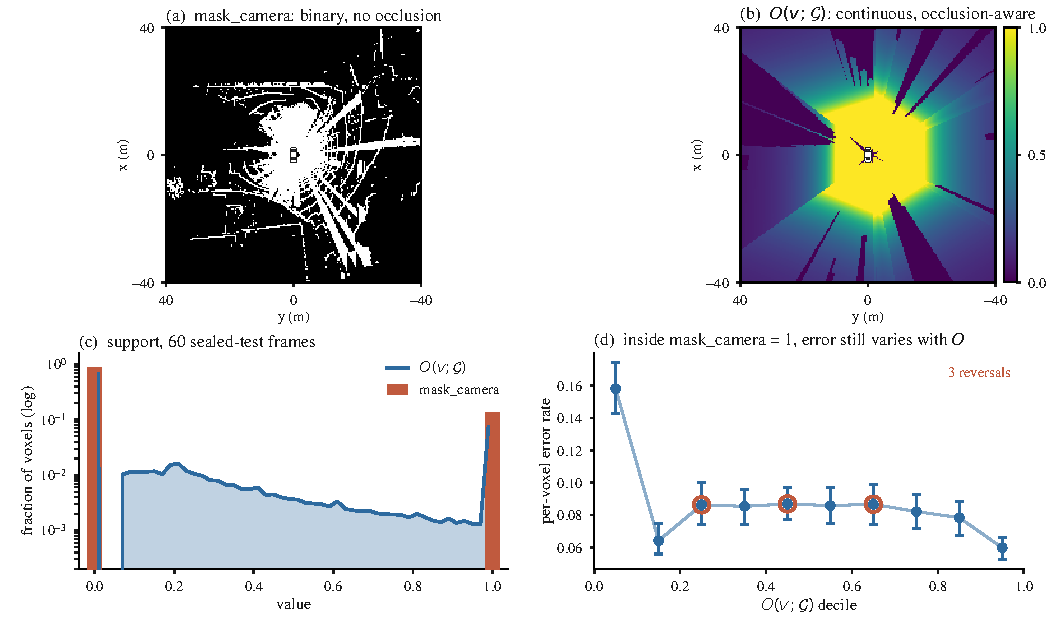
\includegraphics[width=\textwidth]{fig3_whynotmask.pdf}
\caption{\textbf{\texttt{mask\_camera} and $O(v;\mathcal{G})$ are not the
same object.} (a,~b)~One sealed-test frame, token \texttt{4ae9c033}, bird's
eye. The dataset mask is binary and is built offline from the full sensor
suite, including the LiDAR the model never receives; observability is
continuous and resolves occlusion by first-hit ray marching, so the shadow
wedges behind buildings are explicit. (c)~Over \nMvoFrames\ sealed-test
frames the mask takes two values and observability occupies the interval,
log scale. (d)~Restricting to voxels the mask already calls observed, the
per-voxel error rate still varies with $O$ by a factor of
\nMvoRatio: the mask is constant there and ranks nothing. The relation is
not monotone --- \nMvoRev\ deciles rise, circled --- and is consistent with
the H1 contrast in \cref{tab:ledger}, which scores the \emph{calibration
gap} against the same deciles rather than the error rate and counts its own
reversals. The effect is concentrated in the lowest decile. Error bars are paired-frame bootstrap, 95\%.}
\label{fig:maskcam}
\end{figure*}

\subsection{Camera-only occupancy prediction}
Dense occupancy replaced boxes as the camera-only output of choice because
it describes arbitrary geometry. The line runs from the lifting operation
of Lift-Splat-Shoot~\cite{philion2020lss} through the bird's-eye-view
detectors built on it~\cite{huang2021bevdet, li2023bevdepth,
chambon2024pointbev, harley2023simplebev} to BEVFormer's spatiotemporal
attention~\cite{li2022bevformer}. Occupancy methods then split by how they
treat the volume: as semantic scene completion~\cite{cao2022monoscene,
li2023voxformer}, as three orthogonal planes~\cite{huang2023tpvformer}, as
a dual-path transformer~\cite{zhang2023occformer}, as a direct multi-camera
regression~\cite{wei2023surroundocc}, or as forward-backward projection
with a long temporal window~\cite{li2023fbocc}. Later work targets sparsity
and cost~\cite{liu2023sparseocc, lightocc2024, zheng2024monoocc,
kim2025protoocc}, fusion~\cite{li2024gafusion}, and
forecasting~\cite{wang2024occworld, occworldsemi2025}; a survey
covers the area~\cite{occsurvey2024}. Occ3D~\cite{tian2023occ3d} is the
benchmark most are measured on, alongside
OpenOccupancy~\cite{wang2023openoccupancy} and
SemanticKITTI~\cite{behley2019semantickitti}, over
nuScenes~\cite{caesar2020nuscenes} and Waymo Open~\cite{sun2020waymo}.

All of them report mIoU, an average over voxels. An average over voxels
cannot say that some of those voxels were never visible.

\subsection{Uncertainty and failure prediction}
Maximum softmax probability~\cite{hendrycks2017msp} is still the baseline
to beat on in-distribution misclassification, and recent work finds it
competitive with much later proposals~\cite{zhu2024revisiting}. Temperature
scaling~\cite{guo2017calibration} corrects calibration without touching the
ordering, so it cannot change a ranking result. Ensembles and MC
dropout~\cite{lakshminarayanan2017ensembles, gal2016dropout} estimate
epistemic uncertainty at a multiple of inference cost; the
aleatoric-epistemic split has been examined for
vision~\cite{kendall2017uncertainties}. A second family scores a sample
post hoc: feature-space distance~\cite{lee2018mahalanobis}, neighbourhood
agreement~\cite{jiang2018trust}, input perturbation~\cite{liang2018odin},
free energy~\cite{liu2020energy}, and soft-probability
tests~\cite{granese2021doctor}. A third trains the failure predictor
itself~\cite{corbiere2019confidnet, geifman2019selectivenet}. Selective
prediction~\cite{geifman2017selective} gives the evaluation we adopt and
conformal prediction~\cite{angelopoulos2021conformal} the
distribution-free alternative. Dense prediction has its own reliability
literature with the same shape~\cite{derooij2023segreliability,
dreissig2023lidarcalib, blum2019fishyscapes}.

Every method above reads the network. Each is a statement about a
prediction the network produced, which is the limitation
\cref{fig:whyconf} describes and \cref{tab:perclass} measures.

\subsection{Visibility, and the camera mask}
Visibility is not new here and we claim no priority over it.
Occ3D~\cite{tian2023occ3d} ships a camera-observation mask; EvOcc models
unobserved and conflicting space evidentially~\cite{kalble2025evocc};
$\alpha$-OCC studies uncertainty for camera occupancy
directly~\cite{occ2024alpha}; sensor visibility has
been formalised with its own metrics~\cite{borger2022sensorvisibility};
and datasets exist to probe occlusion
specifically~\cite{occludednuscenes2025}. Driving world
models~\cite{rahimi2026mad, xia2026drivelaw, zhu2026dlwm, tan2026lcdrive}
treat geometry as something to reconstruct or condition on. In all of
these, visibility is an input to a model or a mask on a loss.

\paragraph{The camera mask is the closest comparison, and it is one bit.}
Occ3D's \texttt{mask\_camera} marks whether a voxel is observed in the
current camera view, and the obvious objection to this paper is that it
already encodes what we measure. Three differences decide the matter. It
is binary, so inside the mask it is constant and ranks nothing, which is
the regime our comparison operates in. It is built offline from the full
sensor suite, including the LiDAR the model never receives, so it
describes the annotation pipeline rather than what the cameras resolved.
And it marks observation rather than evidence strength: a voxel grazed by
one camera at 40\,m and a voxel filling half an image both read $1$.
\Cref{fig:maskcam} shows the consequence. Restricted to voxels the mask
already calls observed, the per-voxel error rate still varies with
observability by a factor of \nMvoRatio. None of this means the mask fails
at its own job, which is deciding where labels are valid.

What separates this work is the role the quantity plays: held outside the
model and evaluated against the model's own uncertainty, at three
granularities, with the geometry source stated and both choices reported.

\section{Geometric Observability}

A camera rig either resolves a volume of space or it does not, and that
fact is settled by the calibration and the scene, not by the network. This
section makes it a number. We first fix the problem setting
(\cref{sec:prelim}), then define the measure (\cref{sec:defn}), then state
what it costs to compute (\cref{sec:compute}), and finally separate the two
sources the scene geometry can come from (\cref{sec:source}), because that
choice decides what the measure can be used for.

\subsection{Problem setting}
\label{sec:prelim}
A camera-only occupancy model takes the images $\{I_i\}_{i\in\mathcal{C}}$
from a calibrated rig of $|\mathcal{C}|=6$ cameras and predicts a class for
every voxel of a fixed grid $\mathcal{V}$ around the ego vehicle. On
Occ3D-nuScenes the grid is $200\times200\times16$ at $0.4$\,m, covering
$\pm40$\,m laterally, with eighteen classes of which one, index $17$,
means \texttt{free}. Write the prediction $\hat{y}(v)$ and the
ground truth $y(v)$.

We study two failure events. A \emph{voxel error} is
$\hat{y}(v)\neq y(v)$. A \emph{missed object} is the stronger event that a
whole annotated instance goes unrepresented: for a ground-truth box
$\mathcal{B}_j$ of a dynamic class,
\begin{equation}
M_j \;=\; \mathbb{1}\!\left[\;\nexists\, v \in \mathcal{B}_j
   \;:\; \hat{y}(v) \in \mathcal{D} \;\right],
\label{eq:miss}
\end{equation}
where $\mathcal{D}$ is the set of dynamic classes. The two events are not
the same question and, as \cref{sec:main} shows, they are not ranked by
the same signal.

A failure-ranking signal is any score $\phi(\cdot)$ computed per voxel or
per object, evaluated by how well it separates failures from non-failures.
The incumbent is the model's own maximum softmax
probability~\cite{hendrycks2017msp}, $\phi_{\textsc{msp}}(v) =
\max_c \hat{p}_c(v)$, negated so that low confidence predicts error. Its
structural limitation is visible in \cref{eq:miss}: when an object is
missed, every voxel inside its box carries a confident vote for
\texttt{free}, so $\phi_{\textsc{msp}}$ is not merely uninformative there,
it points the wrong way. Any signal that is to catch this event cannot be
a function of $\hat{p}$.

\subsection{The measure}
\label{sec:defn}
Let $c_i(v)\in[0,1]$ be how well camera $i$ resolves voxel $v$, and
$s_i(v;\mathcal{G})\in\{0,1\}$ whether the ray from camera $i$ reaches $v$
before anything else in the scene-geometry field $\mathcal{G}$.
Observability is the best evidence any one camera supplies:
\begin{equation}
O(v;\mathcal{G}) \;=\; \max_{i \in \mathcal{C}} \; c_i(v)\cdot
   s_i(v;\mathcal{G}).
\label{eq:obs}
\end{equation}
The maximum rather than a sum encodes that a voxel seen well by one camera
is observed, however many others miss it. Nothing in \cref{eq:obs} reads
$\hat{p}$, or any uncertainty head, or any learned parameter.

\paragraph{Coverage.}
A voxel of side $r$ at depth $d$ along the optical axis of a camera of
focal length $f$ projects to a footprint of roughly $(f r / d)^2$ pixels.
Coverage normalises that by a constant and clips:
\begin{equation}
c_i(v) \;=\; \min\!\left(1,\; \frac{(f_i r / d_i(v))^{2}}{\pi_{\text{full}}}\right),
\qquad \pi_{\text{full}} = 965.0 .
\label{eq:coverage}
\end{equation}
A voxel resolved by at least $\pi_{\text{full}}$ pixels counts as fully
covered; beyond that range evidence degrades as $1/d^2$ rather than
falling off a threshold. This is the measure's only parameter. It was
fixed once before any result in this paper and never retuned per backbone
or per split, and \cref{sec:ablations} varies it over a factor of four.

\paragraph{First-hit visibility.}
Visibility is decided by marching the ray from camera $i$ and asking
whether $v$ is the first occupied cell it meets:
\begin{equation}
s_i(v;\mathcal{G}) \;=\; \mathbb{1}\!\left[\,v = \!\!\arg\min_{u \in \mathcal{R}_i(v),\,
   \mathcal{G}(u)=1} \!\! \lVert u - o_i \rVert \,\right],
\label{eq:firsthit}
\end{equation}
with $\mathcal{R}_i(v)$ the voxels the ray traverses and $o_i$ the camera
centre. The predicate $\mathcal{G}(u)=1$ is the whole dependence on scene
geometry, and \cref{sec:source} is about where it comes from.

\paragraph{Why not a z-buffer.}
Rendering the volume once per camera and reading depths would be far
cheaper, and we tried nine variants of it. All of them decide occlusion
once per voxel, and a voxel can be half-occluded: a pole in front of a bus
removes part of the bus's footprint, not all of it. Resolving that
correctly requires per-pixel first-hit, which is why \cref{eq:firsthit} is
evaluated by ray marching.

\subsection{Computing it}
\label{sec:compute}
The grid, the intrinsics and the extrinsics are identical in every frame;
only $\mathcal{G}$ changes. The traversal order of each ray can therefore
be precomputed once per camera and reused. We build that table in
$6.9$\,s, hold it in $831.6$\,MB, and per frame the marcher becomes a
gather and a prefix test over six cameras. Measured over eight frames this
runs at $0.329$\,s per frame against $1.139$\,s for the direct
implementation, a speed-up of $3.46\times$, and builds the full
$6{,}019$-frame pack in $33$ rather than $114$ minutes, single process on
CPU. The two implementations were compared voxel by voxel over
$30{,}720{,}000$ voxels and disagreed on none.

Cost is $O(|\mathcal{C}|\cdot|\mathcal{V}|\cdot L)$ for an average ray
length $L$, with no dependence on the occupancy model, so the same table
serves any backbone evaluated on the same rig and grid.

\subsection{Where the scene geometry comes from}
\label{sec:source}
\Cref{eq:firsthit} needs to know what else is solid, and that requirement
is not a detail. We evaluate two choices and keep them notationally
distinct throughout, as $O_{\textsc{gt}} = O(v;\mathcal{G}_{\textsc{gt}})$
and $O_{\text{pred}} = O(v;\hat{\mathcal{G}}_{\text{pred}})$.

$\mathcal{G}_{\textsc{gt}}$ is the dense Occ3D ground-truth volume. It is
independent of the occupancy model, which is why the resulting measure
transfers unchanged between architectures, but it is not available on a
vehicle. It is an evaluation-time quantity and every number in
\cref{sec:main} uses it.

$\hat{\mathcal{G}}_{\text{pred}}$ is the model's own predicted occupancy,
thresholded to occupied or free. This one \emph{is} available at inference.
Note that even here observability reads only the hard class decision, never
$\hat{p}$, so the comparison in \cref{sec:main} stays a comparison between
two kinds of information rather than two readings of the same one.
\Cref{sec:deployable} measures what happens under the substitution, and
the answer is negative in a specific and informative way.

\subsection{From voxels to objects}
\label{sec:agg}
The missed-object event of \cref{eq:miss} is defined on a box, so the
signal has to be defined on a box too. For each annotated dynamic instance
we take the voxels whose centres fall inside the oriented box,
$\mathcal{B}_j$, and aggregate:
\begin{equation}
O_j \;=\; \max_{v \in \mathcal{B}_j \,:\, y(v)\in\mathcal{D}} O(v;\mathcal{G}),
\qquad
\phi^{\textsc{msp}}_j \;=\; \max_{v \in \mathcal{B}_j} \max_c \hat{p}_c(v).
\label{eq:agg}
\end{equation}
Both use a maximum, for the same reason and to keep the comparison fair:
one well-resolved voxel is enough to say the rig had evidence, and one
confident voxel is enough to say the model committed. Restricting $O_j$ to
voxels the ground truth assigns to the object keeps the score on the
object rather than on the free space around it; the confidence score is
not restricted, because the model does not know which voxels those are.
Instances with fewer than eight ground-truth voxels are dropped, since
below that the aggregation is dominated by discretisation. This leaves
\nObj\ objects on the sealed test split.

We also report a LiDAR point-count oracle, the number of returns inside
$\mathcal{B}_j$. It sees a modality the model never receives and is an
upper reference rather than a competing method.


\section{Experiments}

The experiments answer four questions in order. Does the measure beat the
dataset's own camera mask at ranking error (\cref{sec:h2})? Does its value
depend on the granularity of the failure being ranked
(\cref{sec:inversion})? Is it redundant with the model's confidence, or a
second axis? And does it survive the only occupancy field a vehicle
actually has (\cref{sec:deployable})? Every number is computed on a split sealed before method
development, and every contrast was specified before its data existed.

\subsection{Setup}
\paragraph{Model and data.}
FB-OCC r50 with temporal fusion on Occ3D-nuScenes, $200\times200\times16$
voxels at 0.4\,m, 18 classes. We measure mIoU $38.90$ against a
published $39.1$, so the checkpoint reproduces.

\paragraph{The sealed split.}
The 150 validation scenes are partitioned once into a development half and
a held-out test half of \nScenes\ scenes, recorded under digest
\splitdigest. Method development used the development half only; the test
half was opened once. A single module is the source of truth for the
split, and every script and every CI gate reads it from there.

\paragraph{Statistics.}
AUROC~\cite{hanley1982roc} by exact histogram on quantised scores; the
paired scene bootstrap~\cite{efron1986bootstrap} for every interval, which
resamples whole scenes rather than voxels because voxels within a scene are
not independent; risk-coverage and AURC for selective
prediction~\cite{elyaniv2010selective, geifman2017selective}; ECE in 15
bins~\cite{naeini2015ece}. Every contrast reported in this paper was
specified before the corresponding data existed, in the sense
of~\cite{nosek2018preregistration}.

\subsection{Main results}
\label{sec:main}

\paragraph{Observability outranks the camera mask.}
\label{sec:h2}
Scoring per-voxel error inside \texttt{mask\_camera}, where the mask is
constant and therefore ranks nothing, observability reaches an AUROC of
$0.6321$. The contrast H2 against the mask is
\Hii\ \HiiCI\ on the test half, and $+0.0534$ on the full 150 scenes; the
test figure is the one we quote, and the two are given together so the
difference cannot be mistaken for a selection effect.

This is a modest effect in absolute terms and we do not inflate it. Its
interest is that it is obtained by a quantity that costs no training, reads
nothing from the network, and is available before the forward pass.

\subsection{The granularity inversion}
\label{sec:inversion}

\paragraph{What counts as a miss.} For a ground-truth box $B_j$ of class
$y_j$ with predicted labels $\hat{y}$:
\begin{align}
M_j^{\text{any}} &= \mathbb{1}\!\left[\;\nexists\, v \in B_j :
   \hat{y}(v) \neq \textit{free}\;\right], \label{eq:missany}\\
M_j^{\text{dyn}} &= \mathbb{1}\!\left[\;\nexists\, v \in B_j :
   \hat{y}(v) \in \mathcal{D}\;\right], \label{eq:missdyn}
\end{align}
with $\mathcal{D}$ the dynamic classes. We call $M^{\text{any}}$ the \textbf{strict miss}, nothing at all
predicted inside the box, and $M^{\text{dyn}}$ the \textbf{dynamic miss},
nothing \emph{movable} predicted there, so a box filled with predicted road
surface counts as a miss. The second is the one a planner cares about and
the terms are used consistently below. We report
$M^{\text{dyn}}$ and give $M^{\text{any}}$ beside it, because the choice
changes the rate and a reader should see both. Boxes with no LiDAR return
are excluded, and only boxes holding at least one ground-truth voxel of
their own class are scored.

\Cref{fig:qualitative} is one such object in full: the ground truth
contains a bus, the prediction contains no dynamic class anywhere inside
its box, and the observability field is near zero over the same cells. The strict and
dynamic criteria agree on that example; they disagree on boxes the model
fills with static classes, which is why both are reported.

\paragraph{Two rates, two conditionings.} Across all dynamic objects in the
test split, $19.3\%$ are missed under $M^{\text{dyn}}$. \emph{Conditional on
the object's voxels having zero observability} it is \missHi, and at full
observability \missLo\ (\cref{fig:teaser}b). The figures are not in tension
and we state the conditioning each time.

At the voxel level, maximum softmax probability reaches \voxMSP\ against
observability's \voxObs. At the frame level the ordering holds but
narrows, \frmConf\ against \frmObs. At the object level it reverses:
observability reaches \objObs\ against confidence's \objMSP, a gain of
\objDelta\ \objDeltaCI\ over \nObj\ objects in \nFrames\ frames.

A LiDAR point-count oracle reaches \objOracle. It counts returns inside the
ground-truth box in the current sweep and sees a modality the model never
receives, so it is an upper reference, not a competitor. The paired contrast
is $-0.0121$ $[-0.0289, +0.0052]$: observability is \emph{statistically
indistinguishable} from it on this test set, which is weaker than matching
it and is what the interval supports.

% generated by scripts/paper/table1_perclass.py -- do not edit
\definecolor{odfmshade}{gray}{0.93}
\definecolor{swcar}{HTML}{3182BD}
\definecolor{swtruck}{HTML}{D62728}
\definecolor{swbus}{HTML}{FFD700}
\definecolor{swtrailer}{HTML}{8B4513}
\definecolor{swconstructionvehicle}{HTML}{40E0D0}
\definecolor{swpedestrian}{HTML}{FF0000}
\definecolor{swmotorcycle}{HTML}{808000}
\definecolor{swbicycle}{HTML}{FFC0CB}
\begin{table}[t]\centering\footnotesize
\setlength{\tabcolsep}{2.05pt}
\caption{\textbf{Per class, object level, sealed test split.} \emph{missed} is the fraction of annotated objects the model never predicts. AUROC columns rank that event. \textsc{oracle} counts LiDAR returns inside the box and therefore sees a modality the model does not; it is an upper reference, not a competitor. Observability wins on the two largest classes and loses on trailer and bicycle, and both losses are printed.}
\label{tab:perclass}
\begin{tabular}{llrrccc>{\columncolor{odfmshade}}c}
\toprule
& Class & $n$ & missed & \multicolumn{3}{c}{AUROC $\uparrow$} & obs$-$conf \\
\cmidrule(lr){5-7}
& & & & conf. & obs. & \textsc{orac.} & $\Delta$ \\
\midrule
\textcolor{swcar}{$\blacksquare$} & car & 22,096 & 11.8\% & 0.681 & \textbf{0.832} & 0.786 & \textbf{+0.152} \\
\textcolor{swpedestrian}{$\blacksquare$} & pedestrian & 10,407 & 36.2\% & \textbf{0.711} & 0.707 & 0.739 & -0.004 \\
\textcolor{swtruck}{$\blacksquare$} & truck & 3,956 & 11.6\% & 0.696 & \textbf{0.786} & 0.765 & \textbf{+0.089} \\
\textcolor{swtrailer}{$\blacksquare$} & trailer & 1,056 & 11.5\% & \textbf{0.776} & 0.553 & 0.630 & -0.198 \\
\textcolor{swmotorcycle}{$\blacksquare$} & motorcycle & 1,011 & 25.4\% & 0.673 & \textbf{0.720} & 0.714 & +0.047 \\
\textcolor{swbicycle}{$\blacksquare$} & bicycle & 982 & 33.2\% & \textbf{0.820} & 0.708 & 0.723 & \textbf{-0.115} \\
\textcolor{swbus}{$\blacksquare$} & bus & 814 & 13.3\% & \textbf{0.731} & 0.723 & 0.744 & -0.001 \\
\textcolor{swconstructionvehicle}{$\blacksquare$} & construction vehicle & 541 & 48.2\% & \textbf{0.729} & 0.646 & 0.656 & -0.087 \\
\midrule
& \textbf{all dynamic} & 40,863 & 19.3\% & 0.719 & \textbf{0.762} & 0.774 & \textbf{+0.043} \\
\bottomrule
\end{tabular}
\end{table}


\Cref{tab:perclass} breaks this down. Observability wins decisively on
car, the largest class by a factor of two ($+0.152$), and on truck
($+0.089$). It loses on trailer ($-0.198$) and bicycle ($-0.115$), and
ties on the rest. Both losses are consistent with the mechanism rather
than against it: a trailer is large enough that some part of it is almost
always observed, so observability is near-constant across the class and
has little left to rank, while the model's confidence still varies.

\paragraph{Object-level baselines.}
\label{sec:baselines}
A single confidence baseline is not enough to support the claim, so we score
every signal we can read from the same predictions on the same objects:
\begin{center}\small
\begin{tabular}{llc}
\toprule
& Signal & AUROC $\uparrow$ \\
\midrule
\multirow{4}{*}{\rotatebox{90}{\scriptsize model}}
& max softmax probability          & 0.7193 \\
& mean confidence in box           & 0.5409 \\
& mean top-1 minus top-2 margin    & 0.5202 \\
\midrule
\multirow{2}{*}{\rotatebox{90}{\scriptsize geom.}}
& range from ego                   & 0.6660 \\
& observability $O_{\textsc{gt}}$  & \textbf{0.7623} \\
\midrule
& LiDAR points in box \textsc{(oracle)} & 0.7745 \\
\bottomrule
\end{tabular}
\end{center}
The model-derived family is not close to exhausted by maximum softmax, but
it is bounded by it: the best of the three reaches 0.7193 and the other two
sit near chance, because inside a box the model never populated there is
very little for any output statistic to vary over. Entropy and an energy
score require the full class distribution, which our export does not retain,
and MC-dropout and ensembles require additional forward passes, so all four
remain untested here.

\subsection{The geometry source}
\label{sec:deployable}
The result above uses $\text{occ}_{\text{gt}}$ and is a statement about an
evaluation-time measure. We rebuild observability with
$\text{occ}_{\text{pred}}$, changing nothing else: same marcher, same
$\pi_{\text{full}}$, same sealed split. The acceptance criterion was
registered before the run -- the paired interval on
$\mathrm{AUROC}(\text{obs}_{\text{pred}}) - \mathrm{AUROC}(\text{MSP})$ at
object level must exclude zero.

\textbf{It does not survive.} On a pre-declared subsample of 800 test
frames (seed fixed before the run), 10{,}790 objects in all 75 test scenes:
\begin{center}\small
\begin{tabular}{lc}
\toprule
Occluder for $s_i$ & AUROC $\uparrow$ \\
\midrule
$\text{occ}_{\text{gt}}$ \;(evaluation-time) & \textbf{0.7649} \\
MSP \;(no geometry at all)                   & 0.7184 \\
$\text{occ}_{\text{pred}}$ \;(deployable)    & 0.6708 \\
\bottomrule
\end{tabular}
\end{center}
Paired scene bootstrap: $\text{occ}_{\text{gt}}$ reproduces the headline on
this subsample, $+0.0464$ $[+0.0193, +0.0733]$ over MSP, which confirms the
subsample is not the cause of what follows. The deployable form is
$-0.0477$ $[-0.0828, -0.0135]$ \emph{below} MSP, and
$-0.0936$ $[-0.1113, -0.0761]$ below its own evaluation-time counterpart.
The deployable substitution therefore does not preserve the object-level
advantage, and the next subsection isolates why.

\begin{figure*}[t]
\centering
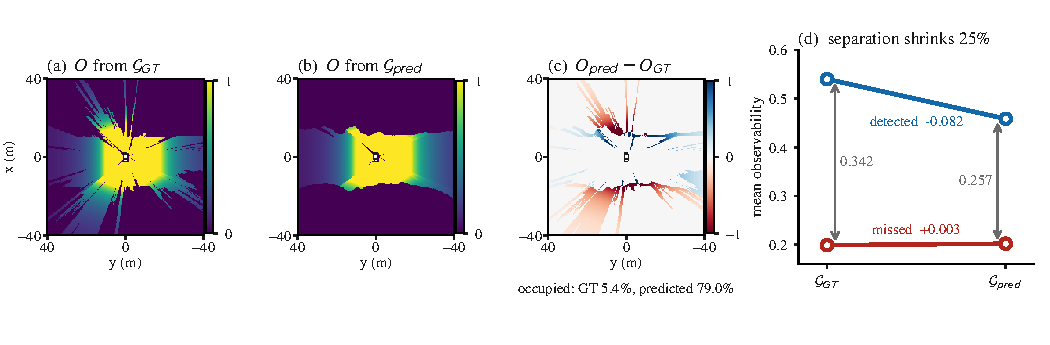
\includegraphics[width=\textwidth]{fig5_deployability.pdf}
\caption{\textbf{What changes when the occluder is predicted.}
(a)~Observability resolved against the ground-truth volume, one sealed-test
frame, token \texttt{90c191b4}. (b)~The same frame resolved against the model's
own predicted occupancy, same colour scale: that field calls 79.0\% of
voxels occupied against 5.4\% in the ground truth, so it casts far more
shadow. (c)~Their difference. Red is observability \emph{lost} to the
substitution, and it dominates: this is over-occlusion, not the circularity
one would predict. (d)~The measured mechanism over 10{,}790 objects.
Observability at \emph{missed} objects is unchanged, while at
\emph{detected} objects it collapses, so the separation between the two
shrinks by a quarter and the ranking degrades. Object-level AUROC falls
from $0.765$ with $\mathcal{G}_{GT}$ to $0.671$ with $\mathcal{G}_{pred}$,
below the $0.718$ of plain softmax.}
\label{fig:deploy}
\end{figure*}

\paragraph{Which side of the comparison moves.} The intuitive explanation
is that a missed object, being predicted free, stops occluding, so the ray
passes through and observability is falsely \emph{high} exactly where we
need it low. That explanation is wrong, and the per-object means say so
(\cref{fig:deploy}c):
\begin{center}\small
\begin{tabular}{lccc}
\toprule
mean observability & $\text{occ}_{\text{gt}}$ & $\text{occ}_{\text{pred}}$ & $\Delta$ \\
\midrule
missed objects   & 0.1987 & 0.2017 & $+0.0030$ \\
detected objects & 0.5402 & 0.4586 & $\mathbf{-0.0816}$ \\
\midrule
separation       & 0.3415 & 0.2569 & $-25\%$ \\
\bottomrule
\end{tabular}
\end{center}
Observability at missed objects is unchanged. What collapses is
observability at \emph{detected} objects, and the ranking degrades because
the top of the scale falls rather than because the bottom rises.

The cause is density. Predicted occupancy is far coarser than the
ground-truth volume --- over 60 sampled frames the occupied fraction is
$0.579$ against $0.052$, a factor of $11$, and $37\times$ on the frame in
\cref{fig:deploy} --- so a great many more rays are stopped. Mean
observability on that frame falls $41\%$ and the zero-observability
fraction rises from $48.9\%$ to $77.7\%$. The measure saturates toward zero
and loses the range it needs to discriminate. This is over-occlusion, not
lost evidence.

That distinction matters for what comes next. An evidence-erasure failure
would be circular and unfixable; an over-occlusion failure is a property of
\emph{this} occupancy field, and a sparser, better-calibrated source of geometry independent of the
occupancy model is not ruled out by this result. Monocular metric-depth
foundation models are the obvious candidate~\cite{bochkovskii2024depthpro,
hu2024metric3dv2, depthanyprior2025}: they run at inference, and
they do not inherit the occupancy model's errors, so a pedestrian that
model drops still has a surface in the depth map. A prior map or a second
modality would serve the same role. We have tried none of them and claim
nothing about them.

\begin{figure*}[t]
\centering
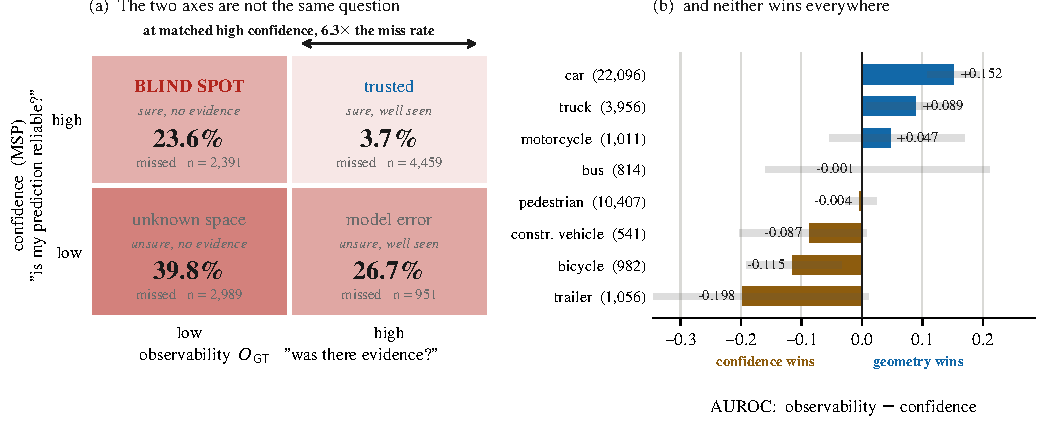
\includegraphics[width=\textwidth]{fig6_quadrant.pdf}
\caption{\textbf{Confidence and observability are different axes,
populated with real objects.} (a)~Test objects split at the population
medians, $O$ $0.36$ and MSP $1.00$ --- more than half of all objects carry
the maximum softmax value, which is the problem the paper starts from;
shading tracks the miss rate. The taxonomy one would draw is not what the
data gives: the worst cell is low confidence with low observability, not
high confidence with low observability. What the data does support is the
paper's claim. Holding confidence \emph{high} and varying observability
gives $23.6\%$ against $3.7\%$ missed, a $6.3\times$ difference at matched
confidence, so the two axes are not redundant. (b)~Per class; bars are the
paired scene-bootstrap mean and rules the 95\% interval. Observability
wins decisively on car and truck, ties on pedestrian and bus, and loses on
construction vehicle, bicycle and trailer. Neither signal dominates, and
we report the losses at the same size as the wins.}
\label{fig:quadrant}
\end{figure*}

\subsection{Analysis}

\paragraph{The two signals are not redundant.}
If observability were merely a noisy restatement of confidence, holding one
fixed would flatten the other. It does not (\cref{fig:quadrant}a). Among
objects the model is \emph{confident} about, those in the low-observability
half are missed $23.6\%$ of the time against $3.7\%$ in the
high-observability half, a factor of $6.3$ at matched confidence. The
reverse also holds, so neither axis subsumes the other.

One number in that figure deserves its own sentence: the median
maximum-softmax value over all test objects is $1.00$. More than half of
every annotated object in the split sits at saturated confidence. A score
that is maximal for the median case cannot separate the median case from
anything, and that is the structural reason the object-level comparison
goes the way it does.

\paragraph{A caveat against our own headline.} The ground-truth volume is
sparse partly because unobserved space is labelled free, and an occluder
set that sparse may \emph{under}-occlude, which would make
$\text{occ}_{\text{gt}}$ optimistic. We have not quantified this and state
it because it cuts against us.



\paragraph{The combined score.}
Where a combined score appears it is a logistic regression on four features,
fitted on the development half and applied unchanged to the test half:
\begin{equation}
S(v) = \sigma\!\big(w^{\!\top}
  [\,\mathrm{logit}\,p_{\max}(v),\; m(v),\; \mathrm{obs}(v),\; d(v)\,] + b\big),
\label{eq:combined}
\end{equation}
with $p_{\max}$ the maximum softmax probability, $m$ the top-1 minus top-2
margin and $d$ range from ego. No weight is tuned on the test half.

\paragraph{Downstream: selective prediction.}
A ranking score is only useful if abstaining on its worst-ranked fraction
actually lowers risk. Measuring area under the risk-coverage curve
(AURC, lower is better) on the sensor-only volume:
\begin{center}\small
\begin{tabular}{lc}
\toprule
Score & AURC $\downarrow$ \\
\midrule
confidence alone                & 0.2526 \\
confidence + \texttt{mask\_camera} & \textbf{0.2128} \\
confidence + observability      & 0.2160 \\
observability alone             & 0.3156 \\
\texttt{mask\_camera} alone     & 0.3542 \\
\bottomrule
\end{tabular}
\end{center}
Adding observability to confidence reduces AURC by
$0.0365$ $[0.0307, 0.0425]$, which holds. Against
confidence plus \texttt{mask\_camera} it is $-0.0033$
$[-0.0051, -0.0015]$: \textbf{observability loses this comparison, and the
interval excludes zero.} We report it because an oracle mask built from the
full sensor suite offline ought to win a volume-level abstention test, and
because the object-level result in \cref{tab:perclass} is not weakened by
it. The two measure different things, and only one of them is available on
a vehicle.

\subsection{Ablations}
\label{sec:ablations}
% generated by scripts/paper/table4_ledger.py -- do not edit by hand
\begin{table*}[t]
\centering\footnotesize\setlength{\tabcolsep}{4pt}
\caption{\textbf{All measured contrasts.} Paired scene-bootstrap means with 95\% intervals on the sealed test split (75 scenes, 3,008 frames); AUROC difference unless noted. Each contrast was specified before its data existed, and every one that was specified is listed here.}
\label{tab:ledger}
\begin{tabular}{@{}ll r@{}}
\toprule
 & Contrast & $\Delta$AUROC [95\% CI] \\
\midrule
\multicolumn{3}{@{}l}{\emph{Per voxel}} \\
H2 & Observability vs.\ \texttt{mask\_camera} & +0.0484 [+0.0390, +0.0584] \\
H4 & Temporal vs.\ instantaneous observability & +0.0156 [+0.0098, +0.0214] \\
H5 & Combined score vs.\ observability alone & +0.2491 [+0.2407, +0.2575] \\
H6 & Combined score vs.\ model confidence & +0.0015 [+0.0009, +0.0022] \\
H1 & Calibration gap vs.\ observability decile & $\rho = -0.433$, 2 reversals \\
\midrule
\multicolumn{3}{@{}l}{\emph{Per object}} \\
E1 & Observability vs.\ model confidence & +0.0432 [+0.0135, +0.0708] \\
E2 & Observability vs.\ LiDAR point-count oracle & -0.0121 [-0.0289, +0.0052] \\
A55 & Predicted-geometry occluder vs.\ model confidence & -0.0477 [-0.0828, -0.0135] \\
\midrule
\multicolumn{3}{@{}l}{\emph{Selective prediction and calibration}} \\
S1 & Observability vs.\ confidence, selective risk & +0.0365 [+0.0307, +0.0425] \\
S2 & Observability vs.\ \texttt{mask\_camera}, selective risk & -0.0033 [-0.0051, -0.0015] \\
R1 & Observability-conditioned vs.\ global recalibration, ECE & +0.0026 [-0.0026, +0.0058] \\
\bottomrule
\end{tabular}
\end{table*}

\paragraph{Temporal accumulation.} Propagating past observability through
ego poses with an exponential half-life, and scoring on the same voxels:
half-lives of $0.5$, $1$, $2$ and $4$\,s give $+0.0080$, $+0.0083$,
$+0.0156$ and $+0.0196$ AUROC over the instantaneous map. The half-life was
fixed at $2$\,s before the run; at that value the interval is
$[+0.0098, +0.0214]$ and H4 holds. The monotone trend to $4$\,s is reported
but was not registered and is not claimed.

\paragraph{Does $\pi_{\text{full}}$ matter?} Less than one might fear,
and the analytic part bounds the empirical part. Coverage is
$\min(1, A_i/\pi_{\text{full}})$, so for a voxel where no camera saturates,
changing $\pi_{\text{full}}$ multiplies every $c_i$ by one constant, leaves
the $\arg\max$ camera unchanged, and is a strictly monotone transform of the
score. Every rank metric here is \emph{exactly} invariant on that set, and
$\pi_{\text{full}}$ can act only through the saturated remainder, which is
$11.9\%$ of in-frustum voxel--camera pairs at the registered value.
Rebuilding observability end to end over a fourfold range and scoring at
object level on 2080 objects:
\begin{center}\small
\begin{tabular}{lcc}
\toprule
$\pi_{\text{full}}$ & object AUROC $\uparrow$ & $\Delta$ \\
\midrule
$500$   & 0.7485 & $-0.0045$ \\
$965$ \;(registered) & 0.7529 & --- \\
$2000$  & 0.7552 & $+0.0022$ \\
\midrule
MSP, same objects & 0.7366 & \\
\bottomrule
\end{tabular}
\end{center}
The spread across $4\times$ is $0.0067$ AUROC, smaller than the effect being
reported, and every value beats MSP. The registered $965$ was derived to
preserve a $16.3$\,m saturation radius before any of these numbers existed,
and no other value is used anywhere in the paper.

\paragraph{Temperature scaling is not a competitor.} It is a monotone
transform of the confidence score, so it leaves every ranking metric in this
paper exactly unchanged. It therefore appears in no ranking table in this paper.

\paragraph{Which term carries the result.} \Cref{eq:obs} has two factors and
a pooling choice, and only one of the three matters. Scoring per-voxel error
on 675 frames across 145 scenes:
\begin{center}\small
\begin{tabular}{lcc}
\toprule
Variant & AUROC $\uparrow$ & vs \texttt{mask\_camera} \\
\midrule
$\max_i c_i s_i$ \;(ours)        & \textbf{0.6755} & $+0.0575$ \\
sum over cameras                 & 0.6748 & $+0.0568$ \\
no temporal term                 & 0.6755 & $+0.0575$ \\
\textbf{no visibility term} $s_i$ & 0.5908 & $\mathbf{-0.0272}$ \\
\texttt{mask\_camera}            & 0.6180 & --- \\
\bottomrule
\end{tabular}
\end{center}
Pooling by maximum rather than by sum is worth $+0.0007$, which is nothing;
we keep the maximum because it is the one with a reading ("seen well by at
least one camera"), not because it measures better. Dropping the visibility
factor, so that coverage alone decides, costs $0.0847$ AUROC and drops the
score \emph{below} \texttt{mask\_camera}. Resolving occlusion is not a
refinement of this measure. It is the measure.

\paragraph{What the blind volume is made of.} On 1{,}238 frames, $76.6\%$
of ground-truth obstacle voxels fall in volumes with no camera evidence,
which is large enough to deserve an account. Attributing each shadowed
voxel to the surface that casts it, over 400 frames and 169M occluded
voxels: man-made structure $43.9\%$, vegetation $27.9\%$, other vehicles
$10.4\%$, drivable surface $4.3\%$, remainder spread across the rest. The
blind volume is mostly buildings and foliage, with one voxel in ten hidden
behind another car, which is the subset a planner cares about most.

\paragraph{Would a seventh camera fix it?} We
re-ran the geometry with each of six additional camera placements added to
the rig. The best of them, a higher roof mount, recovers $2.23\%$ of those
voxels; a rear telephoto recovers $1.29\%$; no other placement exceeds
$0.8\%$. A voxel counts as recovered when its observability rises from exactly zero
to any positive value. Six placements are a finite search and license no
universal claim; what we can say is that none of the placements evaluated
closes more than a small fraction of the unobserved volume.

\paragraph{Summary of measured contrasts.}
\Cref{tab:ledger} collects every contrast in the paper with its paired
bootstrap interval. Three are negative and are reported with the same
weight as the positive ones: the calibration gap is not monotone in
observability (H1), the mask is marginally better at selective risk than
observability alone (S2), and the predicted-geometry occluder does not
preserve the object-level advantage (A55). The first two are small enough
that they bear on presentation rather than on the claim; the third defines
where the measure applies, which is why \cref{sec:deployable} measures its
mechanism rather than reporting it in passing.





\paragraph{Code and data availability.} The measure, the evaluation harness,
the sealed split and its digest, and the amendment log that fixes every
hypothesis and acceptance threshold before its run are released at
\url{https://github.com/AKilalours/opendrivefm} and mirrored at
\url{https://github.com/AkilanManivannanak/opendrivefm}. Every number in this
paper is written by a named script to a JSON artifact in that repository, and
each table and figure names the artifact it reads.

\section{Conclusion}
Geometric observability, computed from the camera rig and an external
occupancy field with one parameter and no learned component, reveals where
a camera-only occupancy model fails in a way its own confidence cannot.
Its value is not uniform across granularity, and that non-uniformity is the
result: the model's own confidence is the better signal for whether a voxel
is wrong, and the worse signal for whether an object is missing entirely,
because a missed object is a confident prediction of free space. External
geometry has no such blind spot, because it never consults the model.
Rebuilding the same signal \emph{from} the model's own predicted occupancy
behaves differently, and not for the reason one would guess: observability
at missed objects barely moves, while observability at detected objects
collapses, because predicted occupancy is an order of magnitude denser than
the ground-truth volume and shadows regions the rig genuinely sees. That is
a property of the particular occupancy field rather than a circularity in
the idea.

Three limitations bound the claim. (1) The measure reads an external
occupancy field, so in the form evaluated here it is a diagnostic for
camera-only occupancy rather than a runtime monitor; supplying that field
from a source independent of the occupancy model, such as a monocular depth
foundation model~\cite{bochkovskii2024depthpro, hu2024metric3dv2}, is the
obvious next step. (2) Every number is one checkpoint of FB-OCC r50 on
Occ3D-nuScenes, so Occ3D's annotation geometry defines both the ground
truth and the occluder set. (3) We measure ranking quality and selective
risk, not collision rate, and we do not compare against sampling-based
uncertainty baselines, which need forward passes our export does not
retain.

{\small
\IfFileExists{ieeenat_fullname.bst}{%
  \bibliographystyle{ieeenat_fullname}%
}{%
  \bibliographystyle{ieeetr}%
}
\bibliography{opendrivefm_refs}
}

\end{document}
